
\usetikzlibrary{shapes,arrows}

\newcommand{\hoo}[0]{H_2O}

\tikzstyle{decision} = [diamond, draw, fill=blue!30, text badly centered, node distance=3.5cm, inner sep=3pt]
    
    %  text width=15em
\tikzstyle{block} = [inner sep = 10,rectangle, draw, fill=black!10, text centered, rounded corners, minimum height=3.5em,node distance=2cm]
    
\tikzstyle{line} = [draw, -latex']

\tikzstyle{cloud} = [draw, rectangle,fill=orange!40, node distance=5cm,
    minimum height=2em]

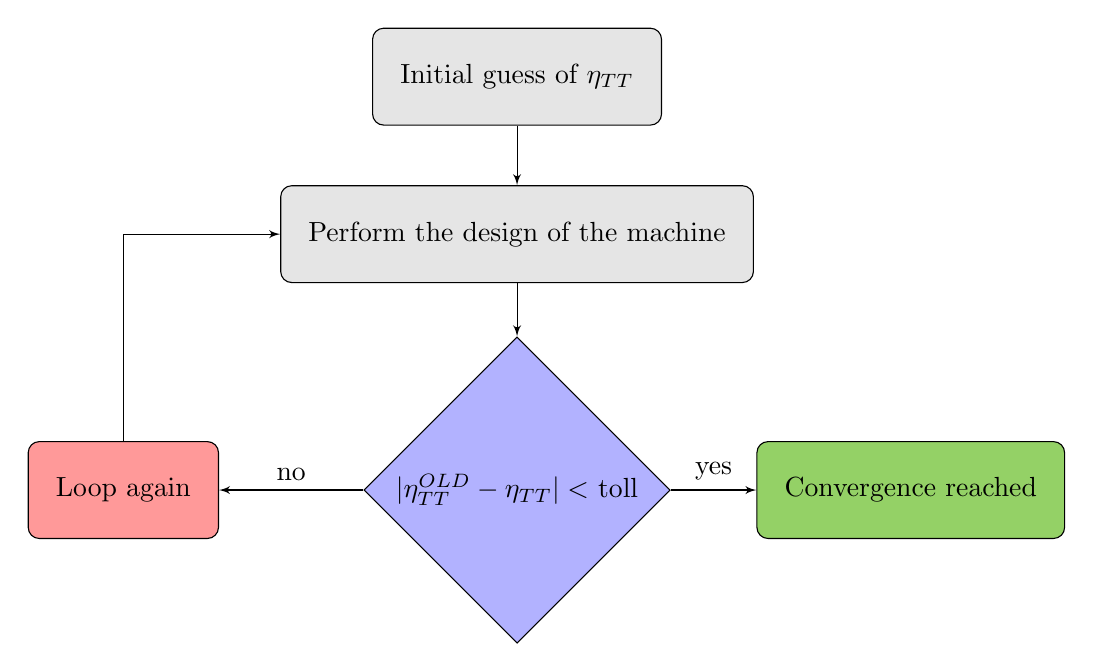
\begin{tikzpicture}
%[node distance = 1cm, auto]

\node [block,align=center] (start) {Initial guess of $\eta_{TT}$};

\node [block, align=center, below of = start] (calculations) {Perform the design of the machine};

%\node [block,align=center] (start2) {Calculate $h_T^{in} = h(p_T^{in}, \text{T}_T^{in})$};

\node [decision, below of=calculations ,align=center, node distance=3.25cm] (decide) {$ |\eta_{TT}^{OLD} - \eta_{TT} |< $ toll};
    
\node [block,node distance=5cm,fill=red!40, left of=decide,align=center] (no) {Loop again};
\node [block,node distance=5cm,fill=green!40!olive!60, right of=decide,align=center] (yes) {Convergence reached};

% now we link together the blocks with arrows

\path [line] (start) -- (calculations);

\path [line] (calculations)--(decide);
\path [line] (decide) -- node[anchor=south] {yes} (yes);
 \path [line] (decide) -- node[anchor=south] {no} (no);
% 
 \path [line] (no) |- (calculations) ;
% 
% \path[line] (c_and_m) --  (dadN) ;
% \path[line] (N) --  (update) ;

\end{tikzpicture}